\section{Cache}

\subsection{IO Elevator}

LLAP offloads I/O and transformation from compressed input to a set of threads referred to as the IO Elevator, as seen in Figure~\ref{fig:elevator}.
The IO elevator interacts with the networked storage in independent threads, which is triggered independently
of the operator pipeline initialization.  This operation starts reading from remote data stores into a cache 
buffer and works as a single split look-ahead pre-fetch, while the plan is initializing multi-vertex inputs
such as broadcast joins.
The 
IO elevator also evaluates any SARGs pushed down to the storage layer, effectively doing those operations 
out of the critical path for latency.
The IO elevator and the operator pipeline work through a small pool of vectorized row-batch buffers, organized
as a producer-consumer queue. The IO elevator places decoded batches into the pool, while the operator pipeline
consumes each batch and returns the batches to the elevator for disposal/reuse.

\begin{figure}[ht]
\centering
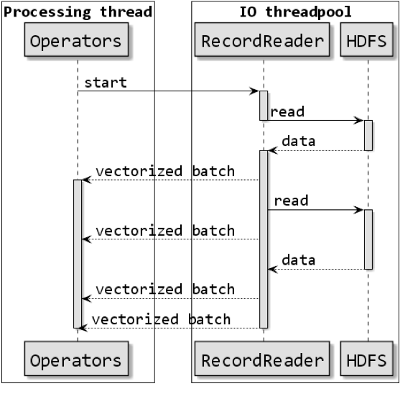
\includegraphics[width=0.8\columnwidth]{figures/elevator.png}
\caption{LLAP: IO Elevator}
\label{fig:elevator}
\end{figure} 

\subsection{Cache Addressing}

LLAP features an off-heap cache as its primary buffer pool for holding incoming data coming into
the IO elevator. The cache is addressed by the IO elevator along two dimensions, one along row-groups usually 10,000 rows and
the other along column order as showin in Figure~\ref{fig:cache_chunks}. The IO elevator reassembles the selected projection
and evaluates the predicates to extract column chunks which can be reconsitituted into the vector row-batches for the operator
pipeline. In case of cache misses, the cache is repopulated with the missing chunks before the reconsistution is performed,
simplifying the codepath and producing an incremental buildup of the cache as a user navigates the data-set along denormalized
dimensions, which is the common pattern the cache optimizes for.

\begin{figure}[ht]
\centering
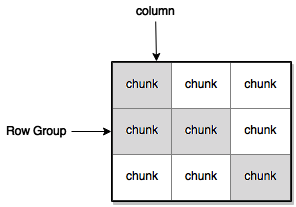
\includegraphics[width=0.8\columnwidth]{figures/cache-groups.png}
\caption{LLAP: Cache addressing}
\label{fig:cache_chunks}
\end{figure} 

LLAP cache holds within the metadata about input files as well as the data. The metadata and index information is cached even 
for data that was never in the cache. This is used to determine the row-groups that have to be loaded and to evaluate predicates
against the metadata before determining cache misses for the column chunks. With this in place, the first scan populates the indexes
in bulk and navigating within a dimension will not have to thrash the cache with column chunks which are effectively index misses.

To maintain validty of the cache, in the presence of updates, the cache lookup uses the HDFS FileId as the unique identifier to 
differentiate files of the same name which have different lineages. For extra strength, this combined with the length of the file
to detect appends to a file and for other fileystems, there are strong consistency equivalents to the FileId such as the ETag 
fields present in blob stores like Amazon S3\cite{S3} or Azure WASB\cite{WASB}. 

\subsection{Cache Policies \& Eviction}

The Cache eviction is also addressed at the same level as the addressing model, with each of those being evicted individually based
on the policy. The policy itself is pluggable, the initial policies available are LRFU and FIFO. The LRFU model is suitable for analytical
workloads with frequent partial table-scans, where retaining frequently used columns can provide cache hits if the projections in the
workload is popular.

\begin{figure}[ht]
\centering
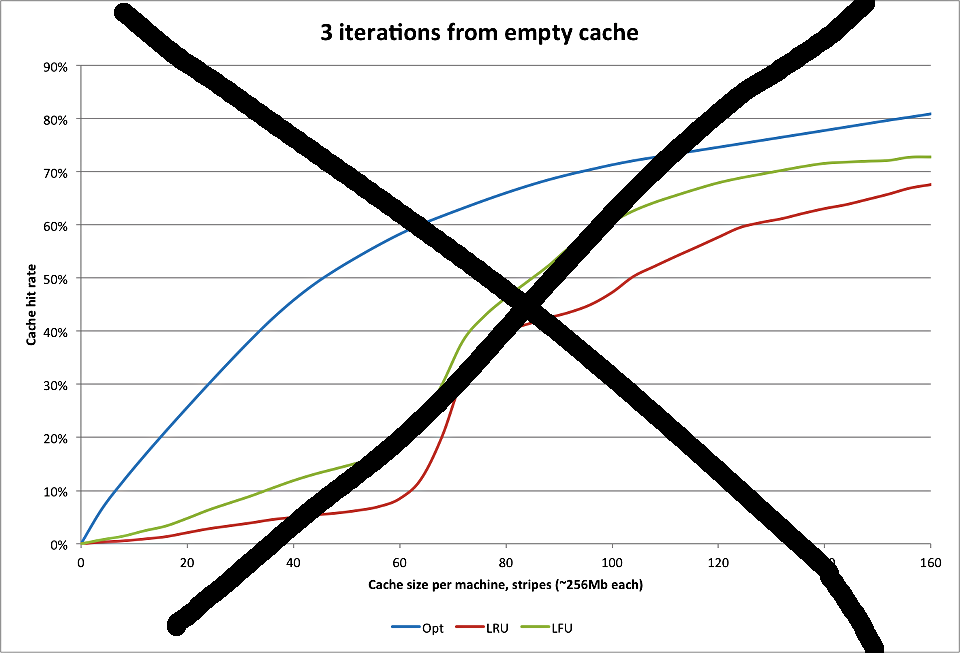
\includegraphics[width=0.8\columnwidth]{figures/evictions.png}
\caption{LLAP: Cache Policies}
\label{fig:eviction}
\end{figure} 

The cache internally uses a BuddyAllocator which handles the fragmentation issues that stem from evictions. The Allocator divies all
allocations into a series of Arenas, with each arena not being bigger than \emph{2Gb} in size due to 32 bit limitations in 
the off-heap APIs. Since the adjacent free blocks are always merged, the cache eviction does not return any memory to the system unlike
the buffer pools, therefore it will reuse the address space for future allocations. 

\iffalse
%% TODO: move to discussions
%% (TODO: discuss fallocate fl_hole_punch as a way of triggering TRIM for garbage).
LLAP does not use the non-volatile nature of NVMe/NVMDIMM
backed caches, preferring to reinintialize the cache on restarts, which removes any potential wear-levelling concerns the BuddyAllocator
brings in by reusing blocks.
\fi

